\section{Ocean tide prediction}
\label{sec:tidesOverview}
%-----------------%
%\begin{quote}
%Tidal prediction is the oldest form of ocean prediction, and is %still the most accurate \citep{Parker:2007wq}. 
%\end{quote}
%-----------------%
\subsection{Why it is worth unpacking ocean tides}
\label{sec:semantics}
The topic of ocean tides is particularly rich in ambiguous and arcane terminology.  
Moreover, it is apparent that this terminology and the underlying concepts lead to miscommunication within operational forecasting.  As operational centres like the Bureau of Meteorology increasingly bring these conventional tidal concepts into the same setting as geophysical simulations that are ever-more `concrete' (introduced in section \ref{sec:concrete}) the need for clarity is amplified.  This potential for confusion is motivates the following exposition of relevant concepts built into the practices of ocean tide prediction.
\newline{}


Tidal methods of analysing and forecasting the ocean have a long legacy in the history of western science.  Economically significant tidal sea level predictions in fact pre-date the whole modern scientific enterprise, and the evolution of the tidal perspective mirrors much of the story of classical continuum physics.

The \citep{Cartwright:2000tt} telling of the history of ocean tide science is illustrative. Remarkably, and perhaps typically, this scientific history of tides never even attempts to pin down a definition of what tide really should mean.  This surely deliberate exclusion stands in stark contrast to the minutiae of historical approaches and formulations and that the history covers.  The absence of definition may be read as an assertion that the history itself is the only meaningful way to frame the scope of tidal science.
\citet{Pugh:1996uz} at least addresses the question of definition explicitly and in doing so casts a very wide net that catches almost anything that can be considered periodic.
\begin{quote}
Although any definition of tides will be somewhat arbitrary, it must emphasise this periodic and regular nature of the motion, whether that motion be of the sea surface level, currents, atmospheric pressure or earth movements. We define tides as periodic movements which are directly related in amplitude and phase to some periodic geophysical force \ldots.
\end{quote}
It is notable that whilst for Pugh periodicity is a key feature of anything that is `tidal', he does not lock this periodicity to astronomy.  Pugh's pragmatic definition appears to be designed to best accommodate the conventional methods of harmonic analysis and sea level prediction that are so well established in operational agencies. Whilst this periodicity-stressing definition sensibly reflects the context of Pugh's text, it is certainly not the only working conceptualisation of what constitutes ocean tides; either within the operational forecasting context or in academic settings. 

In contrast to the periodic definition, most modern authors place the tidal potential in a defining role. Such an emphasis on the tidal potential or Astronomical Tide Generating Forces \ATGP{} reflects a greater regard for dynamics and inputs, as opposed to observed outputs, that is more complimentary to the wider field of geophysical fluid dynamics.  
\citet{Hendershott:1981ub} treats ocean tides as that subset of oceanographic long waves driven by the \ATGP{}.  Notably his discussion is careful with the distinction between dynamics and `practical tide prediction'. But even Henderscott's primarily dynamical perspective is imbued with the cultural interplay of physics and pragmatic prediction; as illustrated by his inclusion of the rather aphysical radiational potential concept associated with the \citet{Munk:1966ts} response method tradition.
The Australian Tide Manual \citep{PCTMSL-sp9} similarly reflects the historical intertwining of tidal physics and practical prediction methods; such that any forcing physics simply provides a backdrop to the singular focus on harmonic prediction.   
A step removed from ocean prediction, \citet{agnew2015} provides a modern physical perspective that both emphasises the core role of the tidal forcing (in this case for earth tides) whilst adopting the well established terminology derived from the long history of ocean tide prediction. A similar emphasis on the physical forcing within the historical perspective is taken by \citet{Flinchem:2000kp} in a  discussion of analysis methods associated with non-stationarity in ocean tide patterns.
The centrality of \ATGP{} be the approach employed in the present work as well.


Further on semantic issues, it is worth highlighting the extent to which the subject of ocean tides raises ostensibly oxymoronic terminology.  
Consider the naming of the a-periodic pole tide, non-stationary tides \citep{Ray:2011tj}, quasi-periodic tidal phenomena \citep{Flinchem:2000kp} or storm tides \citep{Horsburgh:2008gw} each conceptually clashes with the periodic and stationary perspective of conventional harmonic analysis.Put simply, if tides are thought of as period motions how can they be a-periodic?  
A comparable semantic disconnect can arise in circumstances where a tidal prediction exceeds the designated Highest Astronomical Tide level.   
Each of these definitions are sensible in context, but can potentially be a source of miscommunication with the development and delivery of operational forecasts.    Chapter \ref{chp:tideFlavours} proposes measures to partially mitigate such problems.

%-----------------%
\subsection{Common foundation of the \ATGP{}}
Reference to the astronomical tide generating potential (\ATGP{}) is here considered to be the common foundation what is properly considered a tidal method or tidal phenomena.  
The \ATGP{} is an abstraction developed from positional astronomy and classical gravity theory alone.   Perhaps surprisingly for some readers, the underlying role of positional astronomy is formulated in an entirely geocentric, effectively pre-Copernican, framework. 
Figure \ref{fig:tideForceFlow} schematically illustrates the conceptual connections from positional astronomy, to the \ATGP{} and geophysics through to observed sea level .  
Differing treatment of the intermediate parts of this flow chart, the geophysical modelling, effectively comprise the alternative approaches to sea level forecasting.  Of special relevance to the present focus are the details of any decomposition of observed sea level into tidal and non-tidal categories.   The dotted lines connecting nominally non-tidal components indicate that the gravitationally forced response is not the sole factor in discussions of tidal sea level. 
%-----------------
\begin{figure}[!hbt] \centering
    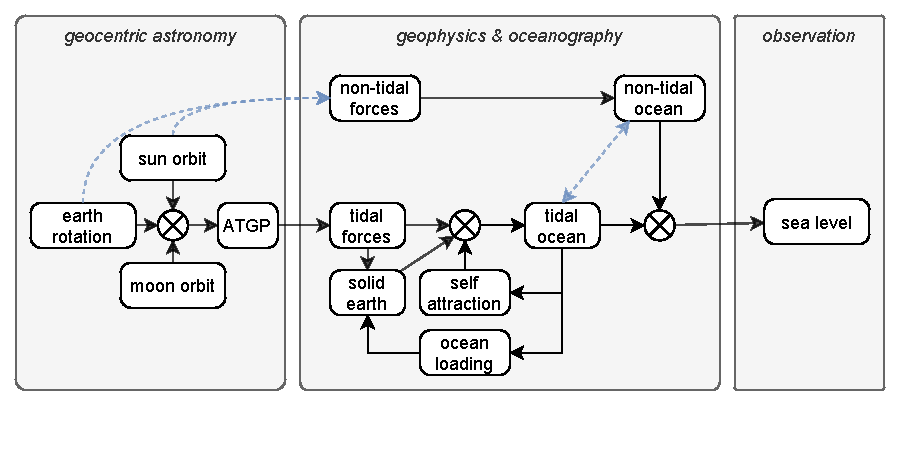
\includegraphics[width=\figwidthFull]{figures/diagrams/tidal_force_flowchart.pdf}
    \caption{Ocean tide flow chart.}{Schematic following \citet{agnew2015}.  Reference to the \ATGP{} is common to tidal analysis and prediction methods, whilst the treatment of tidal/non-tidal connections can differ markedly.}
    \label{fig:tideForceFlow}
\end{figure}
%-----------------
Before expanding on the role of the tidal forcing, the recent work of \citet{10.1016/j.oceaneng.2020.107013} is worth mentioning.   Regardless of the finer details, this observation-based machine learning application to tide prediction is still founded on the connection between positional astronomy and sea level, but simply makes the connection more indirect by relying on easily accessible moon phase data.
%-----------------i
\subsection{Basic development of the \ATGP{}}  \label{sec:basic_potential}
The centrality of the tidal generating potential to sea level forecasting warrants further elaboration, in order to later explicate the manner in which conventional and dynamic sea level forecasts respectively represent tides. 

The \ATGP{} is a mathematical abstraction founded on a consideration of the classical gravitational field near the Earth surface. The temporal variations of gravity in the vicinity of this surface are developed as a function of the geocentric relative positions of the celestial bodies.
For ocean tide applications, only the two celestial bodies, the moon and sun, are considered relevant on the basis of relative contribution to the perceived gravity field changes. It follows that the information required for computation of this lunisolar tidal potential is encapsulated in the celestial positions (ie ephemeris) of the moon and sun alone \citep{agnew2015}.


The full gravity field is defined as a scalar potential in space fulfilling the Laplace equation $\Delta V=0$ \citep[sec 5.3.1]{Urban:2013vl}.  The spatial field $V(\theta,\lambda,r)$ can be formulated in spherical geocentric (ie fixed earth) coordinates as a weighted sum of surface spherical harmonics. As a potential field, contributions from each mass element can be computed separately and linearly superposed.

The specific subset of $V$ attributed to the celestial bodies external to the Earth, but excluding components acting uniformly over the Earth's surface, is defined to be the tidal potential \ATGP{} or $V_T$.
The associated tidal acceleration at any particular point on the earth surface can also be thought as the vector difference between the direct attraction of each celestial body and the orbital acceleration about the Earth-Body barycenter \citep{Wenzel:1997kn}.


The subset $V_T$ of $V$ that is relevant to ocean dynamics is formulated in geocentric coordinates following the convention of \citet{Cartwright:1973em} hereafter \CTE{}, and more recent notation of \citet{Desai:2006wo}:
\begin{equation}
    \eta_{eq} = \frac{V_T(t,\theta,\lambda) }{g} = \sum_{n=2}^{\infty} \sum_{m=0}^{m=n} M_{nm} P_{nm}( \sin(\theta) ) \text{Re} \left [ c^{*}_{nm}(t) e^{im\lambda} \right ]
    \label{eq:VT}
\end{equation}
Where the potential is described only on an idealised spherical earth surface in terms of time, longitude $\lambda$ and latitude $\theta$, as a sum of functions described further below. 

$P_{nm}$ are the associated Legendre polynomials of degree $n$ and order $m$.  Writing $P_{nm}(\sin(\theta))$ gives the surface spherical harmonics.  The fact that the sum begins at $n=2$ is discussed below.
$M_{nm}$ are normalisation factors, that whilst not of direct interest here are noted to follow different conventions between applications \citep{IERS2003}.
Figure \ref{fig:VTmaps} provides a visualisation of the field and a decomposition into spherical harmonics at single snapshot in time.
%-------------------------------
\begin{figure}[!hbt] \centering
    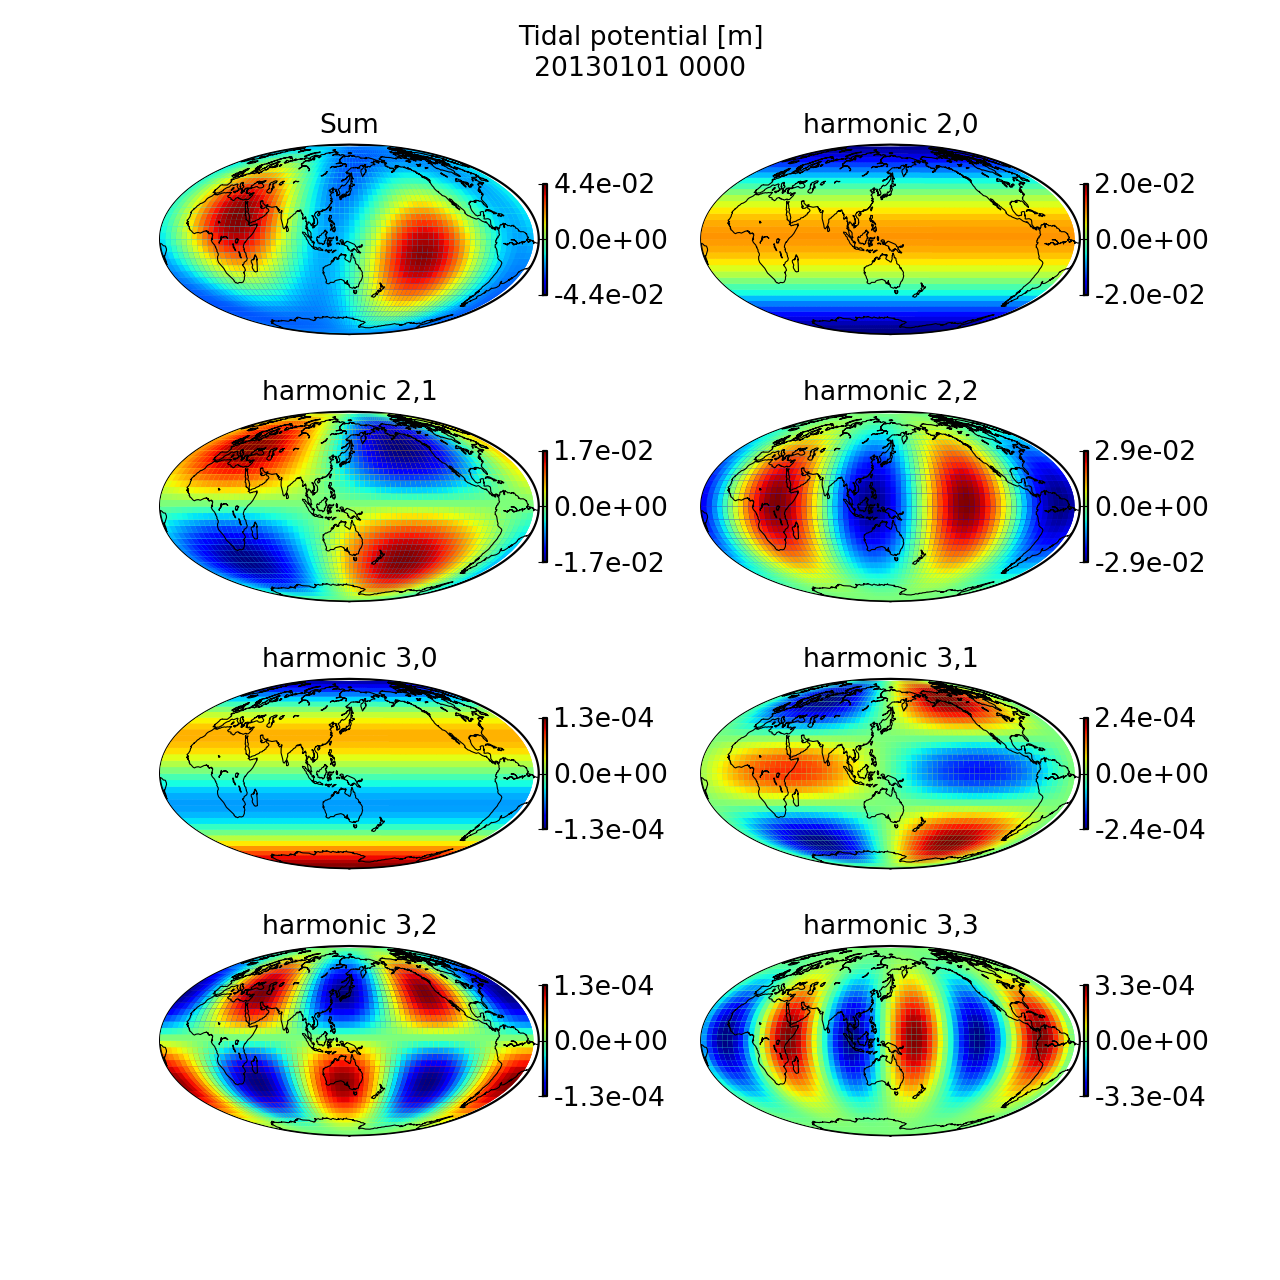
\includegraphics[width=\figwidthBig]{figures/maps/tidal_potential_spatial_20130101_0000.png}
    \caption{Snapshot of global $\eta_{eq}$ field.}{This visualisation illustrates the spatial decomposition into spherical harmonics.  Note the wide variation of relative magnitudes between panels. When comparing to formulations recall that those decompositions are per body; ie an independent set for the moon and sun. }
    \label{fig:VTmaps}
\end{figure}
%-------------------------------
Equation \ref{eq:VT} and the visualisation in \ref{fig:VTmaps} quantify the potential $V_T$ normalised by the standard value for Earth gravity $g$; a quantity defined as the equilibrium tide $\eta_{eq}$.  
A convenience of normalising the potential field as $\eta_{eq}$ is that the quantity has units of height. But this formulation unfortunately invites confusion with actual ocean elevations; whereas the equilibrium tide really only has a very abstract and indirect connection to observed ocean tide heights.
Specifically, whilst useful for formulating the driving force, any direct connection to ocean response is only via the thought experiment of a shallow water idealisation of boundary-free ocean with ``no dynamic effects'' as stated by \citet[Eq 9.8.3]{gill1982atmosphere}; that is, the equilibrium tide is a useless approximation to ocean heights at all expect the longest periods \citep{Egbert:2003jd}.


Equation \ref{eq:VT} represents the spatial decomposition of a surface potential field over the globe.  Of itself, such a formulation asserts nothing specific about the causation of the field.  It embodies no astronomy or ocean dynamics.
Practical implementation of \ref{eq:VT} requires choices regarding the set of harmonics $(n,m)$ to be included and the determination of the time varying complex weights $c_{nm}(t)$.


Only a small set of $(n,m)$ is taken to be relevant for ocean tidal dynamics; in contrast to the thousands of terms utilised for some earth gravity studies. What counts as a relevant ocean subset is generally determined on the basis of the relative magnitude of the terms and the nature of the temporal variation in geographic coordinates.

It is only the horizontal gradient of the potential $\nabla V_T$ that can drive changes in the distribution of ocean mass.   Which to be clear states that the effect of the \ATGP{} on the ocean is to slide mass side-to-side, not directly pull it up.   Furthermore, only temporal changes in this horizontal gradient will effect the non-static ocean distribution. Subsequently degrees $n=0,1$ are not relevant to ocean tides.   This is represented in equation \ref{eq:VT} by the lower limit $n=2$ of the outer sum.
For almost ocean tide applications an upper limit of $n=2$ is taken to be sufficient, or at most $n=3$; again in contrast to some earth gravity studies.  This choice is based on the rapid decline in relative magnitude of each harmonic with increasing $n$ for the luni-solar system - discussed below regarding equation \ref{eq:c}.



The zonal harmonics $(n,m) = (2,0)$ for each body are of particular relevance to the slower patterns of sea level.  Specifically, by having no variation in $\lambda$ these harmonics don't vary geographically with the daily rotation of the earth.   However, the slower changes in the declination of each body do drive an ocean mass response and is associated with both the long period and permanent tides.  
Demarcation of the permanent component of the tide potential is application-dependant.  The details are of particular importance for geodesy and gravity studies \citep[section 5.3.3.2]{Urban:2013vl}.  For ocean forecasting, the role and formulation of the permanent tide becomes relevant in the decomposition of mean sea level for height reduction into a consistent geodetic reference framework \citep{Filmer:2018cu,10.1007/bf02520477}.


All of the temporal variation of $V_T$ is contained in the time series of complex scalar weights $c_{nm}(t)$.
It is significant that these temporal variations of the \ATGP{} for the entire globe can thus be represented by a small number of scalar timeseries - a single complex timeseries for each spherical harmonic included.  For the typical set of harmonics used for ocean tides $(n,m)=(2,1),(2,2)$ this represents a significant compression of spatial information.  
Given the positions in the geocentric reference frame $\theta,\lambda,r$ for both moon and sun, the coefficients are:
\begin{align}
\label{eq:c}
c_{nm}(t) &= a_{nm}(t) + ib_{nm}(t) \nonumber \\
          &= \sum_{b=\text{moon},\text{sun}}    \frac{4 \pi GM_{b}}{g r_{b}}  \frac{(2-\delta_{m0})} {(2n+1)} \left(\frac{a}{r_b} \right)^n    M_{nm} P_{nm}( \sin(\theta_b) ) e^{im\lambda_b}
\end{align}
Where $c_{nm}(t)$ are timeseries of complex numbers equivalently written as pairs of real values $a_{nm}$ and $b_{nm}$ with $i=\sqrt{-1}$.  The normalisation factors $M_{nm}$ are to be consistent with those used for equation \ref{eq:VT}.
Note that $\theta,\lambda$ in Equation \ref{eq:c} are equivalent to the geographic coordinates of the respective sub-body point at a given time. 
Integer $\delta_{m0} = 1$ for $m==0$ and $\delta_{m0} = 0$ for $m \neq 0$.\\
Normalisation factors $M$ are not important to detail here beyond noting that the choice of convention can be relevant to interpretation. The radial scale $a$ is conventional taken as the semi-major axis from the ellipsoidal georeference. 
%---------------------
\begin{figure}[!hbt] \centering
    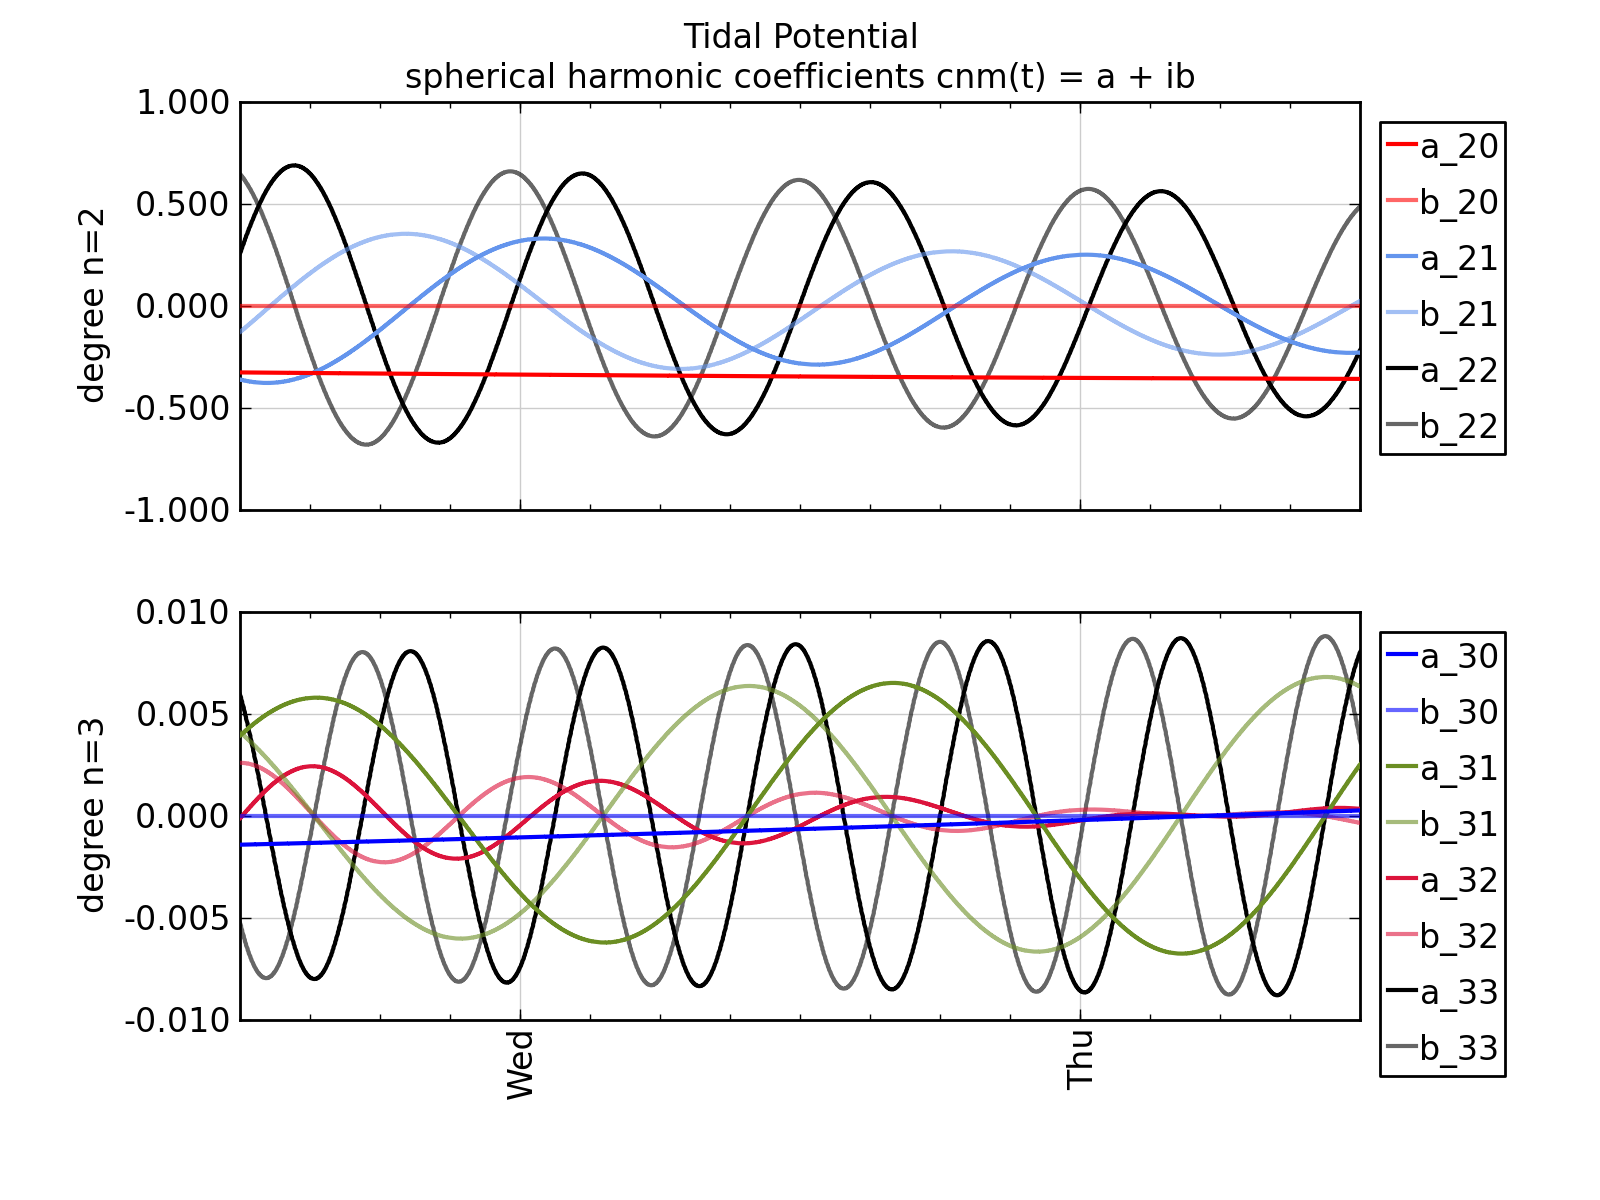
\includegraphics[width=\figwidthBig]{figures/plots/tidal_coeff_timeseries_2days.png}
    \caption{Snapshot of time varying coefficients for the \ATGP{}}
{A short sample of the time varying coefficients $c_{nm}(t)$.  In the upper panel, classification of $c_{2m}$ into long (red), diurnal (blue) and semi-diurnal (black) species is evident.  Note the much smaller magnitude of higher degree harmonics.}
\end{figure}
%---------------------
The rapid decay of the scaling term $\left(\frac{a}{r_b} \right)^n$ with n is the basis for excluding higher degree harmonics from ocean tide applications.  In the case of the Moon, the magnitude of the $n=3$ potential field is more than 2 orders of magnitude smaller than $n=2$.  The associated force also decays, but not quite so rapidly due to the decreasing spatial length scales of the higher harmonics.  This decay is apparent in the colorbars of Figure \ref{fig:VTmaps}\\
The same relative magnitude argument is applied to neglecting more distant celestial masses from formulation of $\eta_{eq}$.

%-----------------%
\subsection{Primary role for temporal variations}
\label{sec:temporal}
The temporal variation of the \ATGP{} is of special relevance to ocean tide prediction.  Inspection of equation \ref{eq:VT} shows that all of this variability is contained within the coefficients $c_{nm}(t)$.  
Any tidal method that applies $c_{nm}(t)$ from a numerical ephemeris in time-space could be said to be \emph{direct}. 
However, transformation of $c_{nm}(t)$ into frequency-space is in fact the basis of many tidal methods.   The highly clustered frequency content of $c_{nm}(t)$ renders this transformation particularly useful.  
Transformation of $c_{nm}(t)$ into frequency space is the basis for \underline{harmonic developments} of the \ATGP{}. Whilst there have been different approaches to performing this development, the common representation is given in Equation \ref{E:harmonic} following \citet{Desai:2006wo} and \citet[Eq 13]{Cartwright:1971iz}.
Furthermore, the ephemeris details for the celestial bodies can be modelled with relatively simple polynomial functions of time; discussed further below. 


It is this harmonic decomposition of the \ATGP{} that leads to the conventional ocean tide practice of harmonic analysis.
%----------------
\begin{equation}
    c_{nm}(t) = \sum_{k} H_{nmk} e^{-i(\theta_{nmk})} = \sum_{k} H_{nmk} e^{-i( t\omega_{nmk} + \beta_{nmk})}
    \label{E:harmonic}
\end{equation}
%----------------
The index $k$ represents a discrete series of tidal components; potentially expanded out to hundreds of terms.  Each component is associated with a discrete point in complex frequency-space with amplitude $H$ and angular argument $\theta_{nmk}$.   For the relevant celestial bodies this argument can further decomposed to time variations at a fixed frequency $\omega$ relative to a reference phase $\beta$.  

Despite a common misconception, it is important to emphasise that equation \ref{E:harmonic} does not represent a Fourier series.  The finite sequence of frequencies $\omega_{nmk}$ are derived from the relative motions of the earth-moon-sun system and do not provide either an orthogonal set of sinusoids nor a complete basis.
Whilst not an orthogonal set, the harmonic decomposition does provide a special list of frequencies that can be ranked by the scalar magnitudes $H_{nmk}$. 

\citet{Doodson:1921kt} introduced a novel and influential system of notation for specifying $\theta_{nmk}$ based on a laborious harmonic decomposition of $V_T$ using Brown's lunar theory; that is, a polynomial model for the lunar ephemeris.  
In the Doodson formulation, all the relevant astronomical information is summarised by code of 6 small integers; together called the Doodson number or argument numbers.   Each position in the code is associated with an fundamental astronomical concept as summarised in Table \ref{T:doodson}.  Doodson codes are in common use across the tidal literature and provide the only useful means of describing tidal components beyond the small number associated with traditional Darwin names such as M2, K1, O1, S2.
Of these traditional names \citet{agnew2015} correctly states that `` [whilst] it is convenient to have a shorthand way of referring to these harmonics; unfortunately, the standard names,  now totally entrenched, ... simply have to be learned as is.''.

There has been some variation of conventions with regard to the exact formulation of Doodson numbers.  One such detail is the avoidance of negative integers in the code by the addition of the arbitrary constant 5 to all integers except $d_1$.   A less common variation involves the use of solar-hour in place of lunar hour $\tau$.  
In essence the Doodson codes provide a compact unique specification, or in practice definition of frequencies relevant to tidal methods.

Whereas the Doodson codes provide a reliable way to describe these tidal frequencies, the mapping to traditional names is unfortunately not always consistent and can lead to errors if transferring parameter data between software platforms; this issue is taken up in chapter \ref{chp:tideFlavours}.


\begin{table}[htp]
\caption{Doodson astronomical arguments.}
{Small integer combinations of these six numbers $d_1 d_2 d_3 d_4 d_5 d_6$ are used to classify tidal components.  Recall that longitudes are celestial, not geographic, coordinates}
\begin{center} 
\begin{tabular}{|c|c|c|}
\hline
Description                            & Argument          & Period\\
\hline
Mean lunar hour                        & $\tau$            & $\sim$ 1 day      \\
Moon mean longitude                    & $s$               & $\sim$ 27 days    \\  
Sun mean longitude                     & $h$               & $\sim$ 1 year     \\
Longitude of lunar perigee             & $p$               & $\sim$ 8.85 years \\
Negative longitude of mean lunar node  & $N^\prime$        & $\sim$ 18.6 years \\
Longitude of Sun mean perigee          & $p_1$             & $\sim$ 20000 years\\
\hline
\end{tabular} 
\end{center}
\label{T:doodson}
\end{table}


Equation \ref{E:doodson} gives the angular argument for a single tidal component $k$ as a function of the 6 astronomical arguments.   As discussed above, the astronomical arguments embody an analytical ephemeris for the Moon and Sun rather than a direct numerical description of these positions.  Polynomial functions of time can be used to estimate each of the 6 arguments close to a given epoch.  The phase adjustment $\delta$ is a convention applied such that the each term in equation \ref{E:harmonic} is written as a cosine, rather than the mixture of sine and cosine terms that naturally follow from the underlying spherical harmonics.

\begin{align}
    \label{E:doodson}
    \theta_{nmk}  &= \left[d_1, d_2, d_3, d_4, d_5, d_6, \delta(n,m) \right] \cdot \left[\tau, s, h, p, N^\prime, p_1, \frac{\pi}{2}   \right]   \nonumber \\
          d_1 &\equiv m \nonumber\\
%\end{align} 
%\begin{equation}
    \delta(n,m) &=  \begin{array}{ll}
                    1 & \mbox{if $n+m$ odd}  \\
                    0 & \mbox{if $n+m$ even} 
                    \end{array}             
%\end{equation}
\end{align} 

Terms are all described in the immediately preceding text.
Some authors formulate these code equivalently by adding an integer offset of 5 to $d_2d_3d_4d_5d_6$ so as to avoid negative numbers.

%-----------------%
\subsection{Other aspects relevant to global coordinates}
\label{S:ATGP_extras}
The essential development of the \ATGP{} in Section\ref{sec:basic_potential} is standard.  However, progressing beyond the basic development towards an ocean forecasting application raises several issues of significance that depend on the details of the application.


\underline{Solid Earth deformation and vertical reference.}  \\
The basic spatial perspective behind the development of the \ATGP{} is the thin shell approximation.  Geocentric coordinates are used.  This is appropriate for writing the potential in general form.  However, when considering the response of ocean dynamics, a vertical relative to the ocean floor is dynamically relevant.  There is a vertical movement of the ocean floor in geocentric coordinates associated with the \ATGP{} of comparable magnitude to the ocean tide which is quantitatively significant to dynamic models; as per \citet{Hendershott:1981ub} and \citet[pp.336]{gill1982atmosphere}.


This elastic response of the earth can be considered to be essentially instantaneous compared to ocean timescales.  Furthermore, the elastic re-distibution of mass associated with this 'earth tide' itself modifies the gravitational field.    By treating the Earth as "spherical, non-rotating, elastic, and isotropic" the solid body response can be encapsulated by a small number of dimensionless Love numbers \citep{agnew2015}.  In the present context each spherical harmonic degree has a single body tide Love number $h_n$ and `induced free space potential' Love number $k_n$ \citep[Sec 5.3.3]{Urban:2013vl}. This has the convenience of formulating the combined direct effects of the solid earth response to the \ATGP{} as a modification to the magnitude of $\eta_{eq}$ shown in equation \ref{eq:love}.  
\begin{equation}
    \eta_{eq} = -(1+k_n-h_n) \frac{V_T}{g} \sim 0.7 \frac{V_T}{g}
    \label{eq:love}
\end{equation}
Where the effect of the Love numbers $k_n$ and $h_n$ is to effectively reduce the nominal magnitude of the equilibrium tide by around $30\%$. 
It is notable that ``the Love numbers for the diurnal tides differ from those for the semi-diurnal and long-period tides because of the free-core nutation resonance'' \citep{Arbic:2004wz}.

The conceptually related, but more complicated, effects of the moving ocean mass itself is discussed below.

\underline{Treatment of self attraction and loading.} \\
The tidal movement of ocean mass has an effect on the solid Earth, and reflexively on the gravitational potential acting on the ocean itself.
From an ocean modelling perspective, elastic compression of the solid earth due to the time varying mass of ocean is referred to as the `load tide'.  The effect of the moving distribution of ocean mass on the gravitation potential field is referred to as `self-attraction'.

Together these effects are lumped together as self-attraction and loading \SAL{}.  They are conceptually distinct from body tides in that \SAL{} is a reflexive function of the time varying spatial distribution of global ocean mass.
Similar effects that vary on tidal timescales are also associated with the time varying distribution of atmospheric mass as well land-based loading from ice,snow and soil moisture.  The value of explicitly distinguishing non-ocean \SAL{} in the context of ocean forecasting is not known, and no publications appear to address this in detail.  It is likely that practical evaluation of \SAL{} for ocean modelling implicitly accounts for some atmospheric effects - especially for the ocean tide associated with pressure forcing S1 and S2.


Similarly to body tide effects, it is possible to formulate \SAL{} as a scaled modification to the astronomical tidal forces.  This is very convenient, but known to be associated with significant inaccuracies \citep{Ray:1998jl}.  The present distribution of \MOM{} makes this so called `$\beta$' approximation.\\
An evaluation of intermediate methods to parameterise SAL is described by \citet{Stepanov:2004up}
In contrast to the $\beta$ scaling approximation, it appears to be quite reasonable to consider \SAL{} as separate pre-calculated body forcing rather than a scaling of $\eta_{eq}$. 
\begin{quotation} \noindent
SAL should be computed by convolution \dots with the Green's function for loading and self-attraction. Since this convolution smoothes out small-scale features, and since large-scale tidal elevations are now well determined over most	of the earth, SAL is in fact now reasonably well known, even where local details of tidal elevations and currents remain uncertain. \citep{Egbert:2002ug}
\end{quotation}


\underline{Time, polar motion and ephemeris.}\\ 
Diurnal Earth rotation and hence time UT1 are effected by tidal effects \citep[sec 8]{IERS2003}.  In addition, conventional UT1 contains discontinuities at leap seconds is not strictly identical to ephemeris time.  For the purposes of ocean forecasting these variations are in general considered negligible and definitions of time are treated as unproblematic.\\


A special case is the \underline{pole tide}. Geocentric coordinates align the polar zenith approximately with the Earths axis of rotation. However, there are continual variations of alignment from the reference axis described by theories of precession and nutation and in general referred to as `polar motion'.   More generally, any changes in the Earth's instantaneous rotation vector can be associated with changes in the gravity field  experienced in surface fixed geocentric coordinates.\\
\begin{quotation} \noindent
Polar motion of the Earth is almost completely described by two harmonic variations of the location of the instantaneous rotation pole with respect to the mean rotation pole: an elliptical motion at an annual period, and an almost circular motion at a period of 14 months. The 14-month variation is a free mode of the Earth referred to as the Chandler wobble and has amplitudes that vary with time. \citet{Desai:2002ev}
\end{quotation}
The gravitational effect due to polar motion can be formulated similarly to the tidal forces as a potential field decomposed into spherical harmonics.
Pole tide effects are included as corrections to altimetry products, but are ignored in standard tide table production.\\
Another phenomena effecting Earth rotation is the Free Core Nutation (FCN).  For the present ocean tidal purposes the FCN will be considered relevant only with regard to the solid earth tides.  The FCN is a factor in defining the  Love numbers in the diurnal band.   Related to this, Desai and Wahr note that the definition of the K1 input amplitude used for solid earth tide algorithms can be inappropriate for ocean applications if compensation for the effects of the FCN resonance are included\citep{Desai:1995je}.



The formulation of the tidal potential in Section\ref{sec:basic_potential} involved only the instantaneous relative positions of the Earth-Moon-Sun system.   These positions are taken from an ephemeris.  In practice, there are two broad classes of ephemeris; analytical and numerical \citep{Wenzel:1997kn}.


An analytical ephemeris provides the relative positions of the Moon and Sun via relatively simple polynomial relations, optimised for a given epoch.  Such analytic ephemeris have been commonly employed for ocean tide studies.   Analytic ephemeris were used initially for computational necessity and more recently for computational convenience.


For modern astronomical purposes numerical ephemerides are now standard.  Prior to 1984 standard ephemeris were based upon \emph{theories}\citep[sec 8.1]{Urban:2013vl}, whereas contemporary ephemeris are created by the application of dynamical equations integrated into the future, after initialisation via assimilation of past observational data.

At the time of writing, the current best estimates for the orbits of the Moon and planets is DE421 \citep{Folkner:2008wm}.   The snapshot visualisation shown in Figure \ref{fig:VTmaps} were calculated based on the application \ref{eq:c} to output of DE421.


The direct application of modern numerical ephemeris to global ocean tide simulations has been demonstrated by for instance \citep{Weis:2008ex} and \citep{10.1007/s10236-016-1016-1}.
However the attractive properties of this approach appear yet to have outweighed the simplicity offered by conventional decomposition approaches.   The ability to isolate named constituents for evaluation is valued for inter-comparisons such as that of \citet{Stammer:2014vh}.
A more accurate ephemeris is likely of less significance to ocean tide hydrodynamics than the conceptual approach regarding the extent to which forcing and response are viewed in frequency space \citep{10.17125/gov2018.ch13}.

A frequency-space view of sea level has arguably come to be more fundamental to tide prediction than the physical foundations of the \ATGP{}; and this topic is addressed next.

%-----------------%
\subsection{Ocean as an LTI System}
\label{sec:LTI}
With historical hindsight it could be said that the success of tidal sea level prediction have been based on treating the ocean as a linear time invariant (LTI) system driven by the \ATGP{}.\footnote{The nomenclature LTI is taken from engineering control theory, not the historically influential Liverpool Tide Institute.}

In essence, the ocean response to tidal forcing is modelled as stationary in frequency space.  Once this time-invariant ``black box'' model has been characterised, astronomical empherides map linearly to sea level predictions.  The details of how the LTI system is characterised and implemented distinguish the variants of tidal analysis and prediction.

Two important aspects of this broad approach were introduced in the late 1700's by Laplace \citep[chpt 7]{Cartwright:2000tt}:
\begin{itemize}
    \item the spectral banded-ness of $V_T(t)$ and the value of a stationary frequency perspective;
    \item application of semi-empirical analysis to simply characterise the expression of complex hydrodynamics. 
\end{itemize}

Modelling the ocean as an LTI system in this manner necessarily takes a frequency-space perspective and assumes model stationarity. \citet{Jay:2003bj} suggest that the long history and apparent value of this perspective has $\dots$
\begin{quotation} \noindent
solidified an opinion that tidal time series (particularly those of surface elevation) are basically stationary, with non-stationary components frequently being regarded as meaningless `noise'.    
\end{quotation}
In fact, as discussed in section \ref{sec:semantics}, frequency-space stationarity is essential to the definition of what is considered tidal in most operational settings.
% little flow chart
\begin{align}
    c_{nm}(t) \Rightarrow & \fbox{Global Ocean}\Rightarrow \mbox{observed response} \nonumber
\end{align}

Time invariance of the LTI in frequency-space means that each input component maps directly to an output response at the same frequency, characterised by an amplitude and phase transformation.   As the LTI characteristics are identified via semi-empirical methods, any hydrodynamics are essentially hidden within the black box and are largely irrelevant.

The core of such a tidal model is schematically shown as a mapping at each distinct tidal frequency:
\begin{align}
    H_{k}(\theta_k) \Rightarrow & \fbox{empirical LTI system} \Rightarrow \mbox{tidal ocean $f(\theta_k)$}  %\nonumber
    \label{eq:LTI}
\end{align}

Conceptualising the global ocean in frequency space raises some peculiarities as characterised by  \citet{Groves:1975ky}: ``by an unfortunate coincidence, the size of the earth, the depth of the ocean, and the rate of earth rotation are such that the frequencies of the free modes of ocean oscillation are intercalated with the frequencies of the tide-generating consitituents''.
For sea level, the different forecasting methods are essentially variants on the  definition of a reference input signal and manner in which the LTI system is formulated.   Following Munk and Cartwright \citep{Munk:1966ts} there are three foci for the problems associated with this conceptualisation:
%\begin{inparaenum}[(i)]
\begin{itemize}
\item the spectral continuum of ocean variation;
\item non-gravitational phenomena; 
\item non-linear interactions.   
\end{itemize}
%\end{inparaenum}

%-----------------%
\subsection{Tidal harmonics and formalisms}
\label{sec:formalisms}
There is no unique approach to implementing the LTI concept of ocean tide prediction. In fact, ``\textit{many organisations have developed their own methods of tidal analysis}''\citep{IOC:2005tj}. But the different approaches or formalisms share the LTI system model discussed above.  
In very broad terms these formalisms fall into basically two categories: harmonic methods and response methods.  
Neither of these concepts actually involve any hydrodynamics. When hydrodynamic simulations of the ocean are undertaken it seems that tidal LTI conceptualisations are at least indirectly involved in one way or another; and this will be apparent in subsequent sections dealing with hydrodynamic and spatial models. 

Within operational authorities, tide prediction is practically synonymous with conventional harmonic methods. It is here that the role of special frequencies (section \ref{sec:temporal}) has come to play a primary role.
``Standard harmonic methods demand little accuracy in the harmonic amplitudes of the [tidal] potential, since they \textit{use only the frequencies} at which the larger amplitudes appear, and certain details on which to base nodal corrections''\citep{Cartwright:1973em} emphasis added.
Recall that the basis for this analysis is not harmonic in the sense of an orthogonal Fourier series, but rather that it follows from the harmonic development of the \ATGP{} as described in section \ref{sec:basic_potential}.    Here again the historical legacy of tidal terminology lends itself to misunderstanding \citep{Cartwright:2000tt}\citep{Parker:2007wq}.


Harmonic methods of sea level prediction are very successful and will continue to be important for years to come, regardless of other advances.  The conventional and routine harmonic analysis of tide-gauge data provides a foundational set of products that is embedded across the whole coastal economy. Tide tables and derived tidal planes (such as LAT) provide ubiquitous references for both land and marine applications. This situation provides some of the difficulties discussed in Chapter \ref{chp:aggregate}, and is elaborated further in  Chapter \ref{chp:tideFlavours}.


At its foundation, harmonic tidal analysis and prediction characterises the ocean response as a LTI system via a finite set of amplitude and phase terms that are identified empirically by the application of timeseries methods.   This concept is stated a little too simply in the Australian Tide Manual as follows: ``\textit{ the purpose of tidal analysis is to represent the water level or current time series by a set of harmonics, or sine waves, each of them having a specific amplitude and phase}''\citep{PCTMSL-sp9}.
Note the emphasis on periodicity rather than dynamics.  More problematic is the fact that this stated purpose is neither universally agreed nor implemented by any tidal agency, as the following discussion will outline.  
The conventional harmonic tide representation of a timeseries is given in equation \ref{eq:cos}.  At face value involves a linear sum of sinusoids with amplitude $A_k$ and phase lag $g_k$ parameters considered to be constants that characterise the LTI system; other terms and complications are discussed below.  
%---------------------
\begin{equation}
    \eta_{tide}(t) = \sum_{k} f_k A_k \cos ( t.\omega_k + g_k + u_k)
    \label{eq:cos}
\end{equation}
Where $\eta_{tide}$ is the time varying tidal signal, $A_k$ and $\omega_k$ are the nominal tidal amplitude and frequency, $g_k$ is a reference phase argument (dependant on the ephemeris epoch) and conventional adjustments $f_k$ and $u_k$ to account for finite record length and are discussed below. 
%---------------------
Significantly, the harmonics involved with such an analysis can only ever be a subset of tidal frequencies arising from the decomposition $c(t) = \sum_{k} H_{k} e^{-i( t\theta_{k})}$.  This limitation comes mainly from the non-orthogonality of the basis functions and the fact that all observational records are of finite length.
Conventional tide practice applies a range of elaborations and work-arounds in order to select the set of analysed components and produce predictions.  
Before discussing any further, the essential steps of the harmonic analysis and prediction process are  illustrated schematically in Figure \ref{fig:tidePractice} and summarised as follows:
\begin{enumerate}
    \item formulation of component set based on various conventions;
    \item empirical projection of an observation record onto the resulting non-orthogonal basis functions;
    \item application of conventions accounting for unresolved frequencies; 
    \item synthesis of tidal timeseries by applying matching conventions.
\end{enumerate}

The practical value of harmonic methods reflects the special significance of sea level variation occurring at tidal frequencies. This value does not rely on simulating ocean dynamics. Rather, the very absence of fluid dynamics is a key strength of harmonic methods. 
A record of historical observations at one place is essentially all that is required, with no need for spatial information or any additional inputs whatsoever.

For almost all ocean-exposed locations, harmonic analysis can reduce the majority of sea level variance in a long observational timeseries to a remarkably short list of numbers; typically mapping several thousand values to a few dozen \citep{Flinchem:2000kp}.  This unique data compression could be better exploited for on-demand delivery services as suggested in chapter \ref{chp:tideFlavours}. 


The standout power of some tidal variations is apparent in the spectra shown in Figure \ref{fig:obsSpectraEg}. 
But conventional practice has developed additional terms that are not directly apparent in the \ATGP{} that have in some locations greatly improved the value of the resulting predictions; in particular for what are called the compound, shallow water or overtide terms. In this case, hydrodynamic reasoning has been applied to select and justify additional terms that could result from the behaviour of depth limited waves and wave-wave interactions.
Any seasonal modulation terms are analogous in the sense that the rational for the LTI model has been extended to account for observed patterns rather than derived solely from the \ATGP{}.
%----------------------
\begin{figure}[!hbt] \centering
	\begin{subfigure}[t]{\figwidthHalf}
	    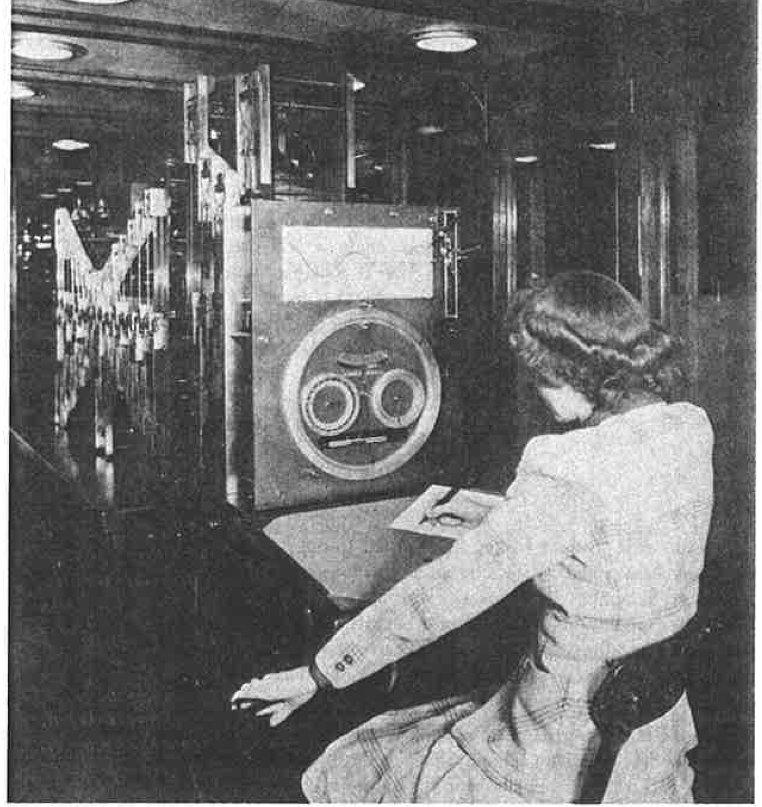
\includegraphics[width=\textwidth]{figures/images/zetler_tidal_computer_lady_1921.png}
	    \caption{Harris-Fischer tide machine circ. 1912 \protect{ \citep{Parker:2007wq} }}
    \end{subfigure}
    \hfill
    \begin{subfigure}[t]{\figwidthHalf}
    	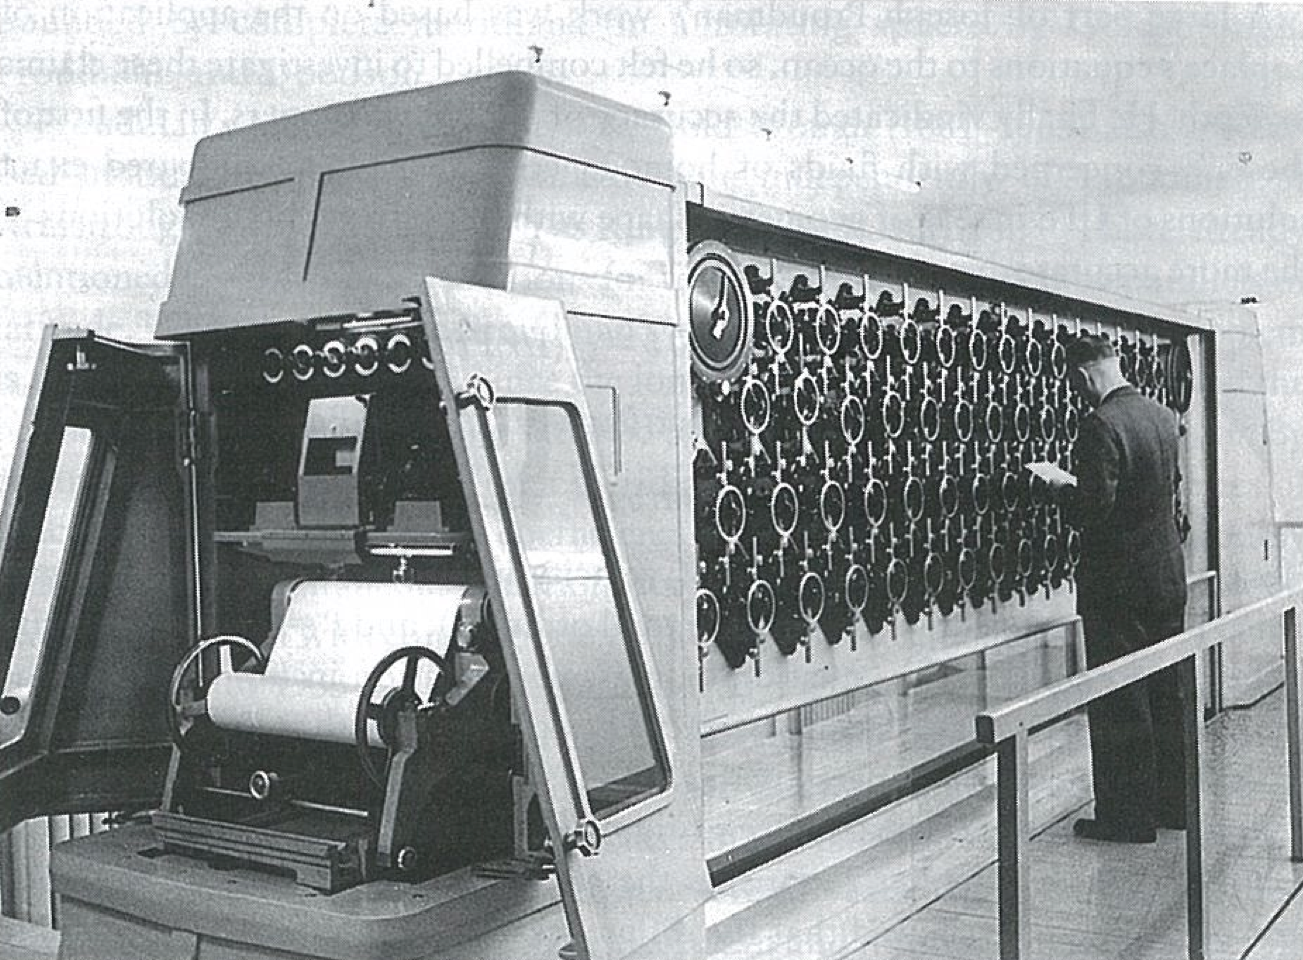
\includegraphics[width=\textwidth]{figures/images/DHI_machine_cartwright_fig11p2.png}
	    \caption{Gezeitenrechenmaschine at DHI circ. 1940 \protect{ \citep{Cartwright:2000tt} }}
	\end{subfigure}
	\caption{Analogue tide machines.}{These instruments embody harmonic prediction and highlight the long operational application of the method.  A finite set of phase and amplitude values are dialled up and the handle turned to generate a prediction timeseries.}
	\label{fig:tide_machines}
\end{figure}
%----------------------
Harmonic analysis can be formulated as an over-determined inverse problem:
%--------------------
\begin{equation}
    \label{E:Axb}   
    \M{A} \V{x}=\V{b} 
\end{equation}
%--------------------
Where $\M{A}$ is a matrix of tidal timeseries basis functions, $\V{x}$ is the analysed tidal solution and $\V{b}$ is an observational record. The tidal basis functions that comprise $\M{A}$ are developed from the combination of the harmonic decomposition of $\eta_{eq}$ and a series of conventions.  The resulting basis is neither orthogonal nor complete. Inclusion of the modulation terms $f_k$ and $u_k$, discussed below, means that the basis functions are not actually sinusoids. The core assumption of stationarity for the finite series of basis functions is equivalent to an assumption that the basis has infinite span in time.   

Practical applications of the harmonic formalism has largely evolved prior to modern cheap computing, and many details can appear somewhat baroque in isolation.  The analogue instruments shown in Figure \ref{fig:tide_machines} serve to highlight this operational history.


The harmonic idealisation effectively operates on infinite basis functions whereas any observational record is of finite length.
Given the close clustering of tidal lines in frequency-space, equation \ref{E:Axb} is poorly conditioned for inversion.   This matrix condition is further degraded by the presence of non-tidal variations. 
Subsequently, practical harmonic analysis procedures must specify which frequencies to include in the basis set and then somehow account for the effects of unresolved frequencies.

At the time of writing the Bureau of Meteorology process does not systematically account for the inversion quality with regard to signal:noise ratios as suggested by \citet{Foreman:2009bg}.
This fact contributes to the potential for overfitting or projection of non-tidal signal onto standard tide predictions that are relevant to later chapters \ref{chp:aggregate} and \ref{chp:tideFlavours}.


Typically arguments regarding the relative magnitude of the harmonic components of $\eta_{eq}$ are used to prioritise candidate frequencies for inclusion with respect to the observational  record length. 
By convention, the effects of clusters of unresolved tidal frequencies are represented by modulation of the basis functions in relationships assumed to map from $\eta_{eq}$.  
In equation \ref{eq:cos} these modulation terms are included as $f_k$ and $u_k$.  These terms are misleadingly known by convention as `nodal corrections', due historically to the close spectral spacing associated with the the lunar nodal regression; differences in $\omega_k$ of about $\frac{1}{18.6}$ years.     These same terms are more informatively called `satellite modulations' by some authors in recognition that the modulation of a constituent term by a very closely spaced spectral cluster arises from terms other than $d_5$. 

Importantly, this nodal modification of basis functions means that the analysis results do not simply represent amplitudes and phases for regular sinusoids.  


There are other aspects in which the routine production of conventional tide tables deviates from the essential matrix inversion, typically to account for observational records that are fragmentary, short or in some way less than ideal.
For instance when additional constants are inferred or directly copied using assumed relationships from either $\eta_{eq}$ or previous analyses.  


To the extent that the non-astronomical phenomena display predictably periodic characteristics, inclusion within the LTI tide model can be to the benefit of a tide prediction; at least when used for conventional tide tables for instance.   
On the other hand, broadband effects that simply project some colour onto tidal basis functions reflect more about the failure of the fitting approach and should rather be accounted for in the forecast error information. Such error information is generally non-existent in standard tide products and at best is implicitly understood in a qualitative sense by users. 

More basically, it is not clear that users of tide predictions are always cognisant of exactly what phenomena conventional predictions represent.    This issue partly motivates chapter \ref{chp:tideFlavours}.
Consider for now the case of seasonal phenomena.   The harmonic decomposition of $c_{nm}(t)$ provides two relatively tiny signals at periods of 1 and 0.5 years - conventionally termed Sa and Ssa.  Despite the insignificance of seasonal terms in the forcing $\eta_{eq}$, conventional predictions frequently assign  disproportionately large values to account for observed patterns.  
Terms that reflect non-tidal seasonal modulation of semi-diurnal components can also be included in standard predictions;such as H1 and H2 in the \citet{Foreman:1977ua} schedule.  There are also  diurnal and semidiurnal sea level signals driven directly by meteorology but coherent with the \ATGP{}. \citet{Ray:2003ui} evaluate \NWP{} representations of barometric tides (ie atmospheric tides) at these frequencies with implications for oceanographic processes.  


Treatment of meteorological versus gravitational influences on observed sea level for terms such as Sa, Ssa, S1 and S2 are a point of difference between conventional harmonic analysis and response methods.  
The \underline{response method}, and it's variations, form a distinct branch of academic tidal analysis that stand in contrast to conventional techniques of harmonic analysis.   This consists of a generalised implementation of the LTI model, in which the ocean response to any input sequence is characterised by empirically determined admittance functions using more general timeseries analysis methods.  
\citet{Munk:1966ts} in fact claimed to be motivated by an application of Ockam's razor to the highly evolved historical baggage of harmonic methods.   
It could be said that response methods simply reflect what physical oceanographers have thought of as `tides' for decades.  This is why harmonic constants are now thought of as just one representation of the idea of a tidal admittance. 
\citep[pp 198]{Cartwright:2000tt} provides the following explanation for why the ostensibly modern response techniques have not displaced conventional practice: 
\begin{quotation} \noindent
    $\dots$ the improvement in predictable variance is numerically small compared with the natural noise in sea level.   Because of this, and the fact that the Response Method is harder for a routine operator to grasp, it has never been adopted for ordinary tide-table production. It remains essentially a research tool for specialists. 
\end{quotation}
But Cartwright's explanation isn't quite the whole story.   
There are benefits for routine production resilience when the product consists of a short list of named parameter values.   The conventions of harmonic constants provide a level of simple intuition that, regardless of prediction skill, are relatively easy to manage in a routine production schedule.
Much more fundamental is the question of the purpose for conducting a tidal analysis at all; and chapter \ref{chp:tideFlavours} argues that delivery of tidal services would be much improved by design choices that do not allow for any ambiguity in this regard.   
Response methods, and its modern extensions such as the orthotide formalism or tidal wavelet techniques, do not target the same outcome as conventional tide prediction.   All may find a useful place in the operational setting as long as relevance for the application is clear. 
Some additional comments on the topic of tidal formalisms are included as Appendix \ref{appendix:tideFormalisms}, but are not essential to the flow of this discussion.


For emphasis, it restated the harmonic and response models contain the same core concept.   Both model the ocean as an LTI system responding to some type of tidal forcing.   Furthermore, both apply assumptions about the smoothness of ocean admittance functions; in the use of inference in the case of harmonic methods.  Indeed \citep[chpt6]{Fu:2001ub} groups both the standard harmonic and convolution formalism as instances of the `response' formalism on this basis.

By definition these LTI methods represent phenomena stationary in tidal frequency-space.   The value of assuming stationarity is the very basis on which tide tables are built. 
Looking beyond this tide-table view of what actually constitutes an ocean tide, there are a great many instances where non-stationary phenomena are categorised as tidal.    For instance, whenever tidal long waves are modulated by transient or secular changes as described by \citet{Devlin:2017hu};   or even the breaking of internal tidal waves \citep{10.3389/fmars.2021.629372}.
The analysis of non-stationary tides span a broad range of literature and applications \citep{Jay:2003bj}.
But it would seem that a singular focus on the stationary model for tide tables has so far prevented such techniques finding regular application within routine operations for forecasting.  

Arguably, the apparently singular harmonic view of operational tide prediction reflects a historical legacy that places little importance on the distinction between the role of tidal methods for forecasting versus for filtering.

%-----------------%
\subsection{Distinguishing forecasts and filtering}

Despite the prominent role of harmonic analysis in tide prediction, direct application to the production of forecasts is not actually the only reason for employing tidal methods in an operational agency.   
The other is to filter, or de-tide, a signal in order to derive a meaningful non-tidal signal.    Whilst it is possible and often convenient to de-tide observed sea level by simply subtracting a standard tide prediction, this is not always fit-for-purpose.
It is consistent to de-tide observations with a standard prediction when the objective is to evaluate the error of the tide prediction itself; conventionally termed a 'tidal residual'.
But when the objective is to remove the variability directly associated with the \ATGP{}, or alternatively to optimally reduce the tidal frequency variability within a sample, then the standard tide prediction is likely not a good choice.

Operational oceanography in the form of \BL{} relies on spatial tide models to de-tide (``correct'') sea level observations from altimeter in order to assimilate the resulting sea level anomaly quantity (SLA).   This de-tiding process has been designed to render the observations compatible with the physics of the model.  But ensuring compatibility is not trivial and  many viable solutions are in production via sources such as RADS \citep{Scharroo:2014vv}.  The details of how the altimeter tidal correction is constructed may have implications for interpretation of the final ocean forecast; long-period tides \citep{Egbert:2003jd} and nongravitational tides \citep{Arbic:2005gv} are highlighted as special points of interest with regard to operational sea level forecasts.

As noted above, the current configuration of \BL{} does not assimilate tide gauge data, though in principle these insitu observations could be reduced to a consistent SLA quantity via appropriate de-tiding; for example as in \citep{Matsumoto:2000tg}.

Figure \ref{fig:residualExample} illustrates how observations de-tided for different purposes produce roughly similar but certainly not identical anomaly signals. 

%-------------------------
\begin{figure}[!hbt] \centering
    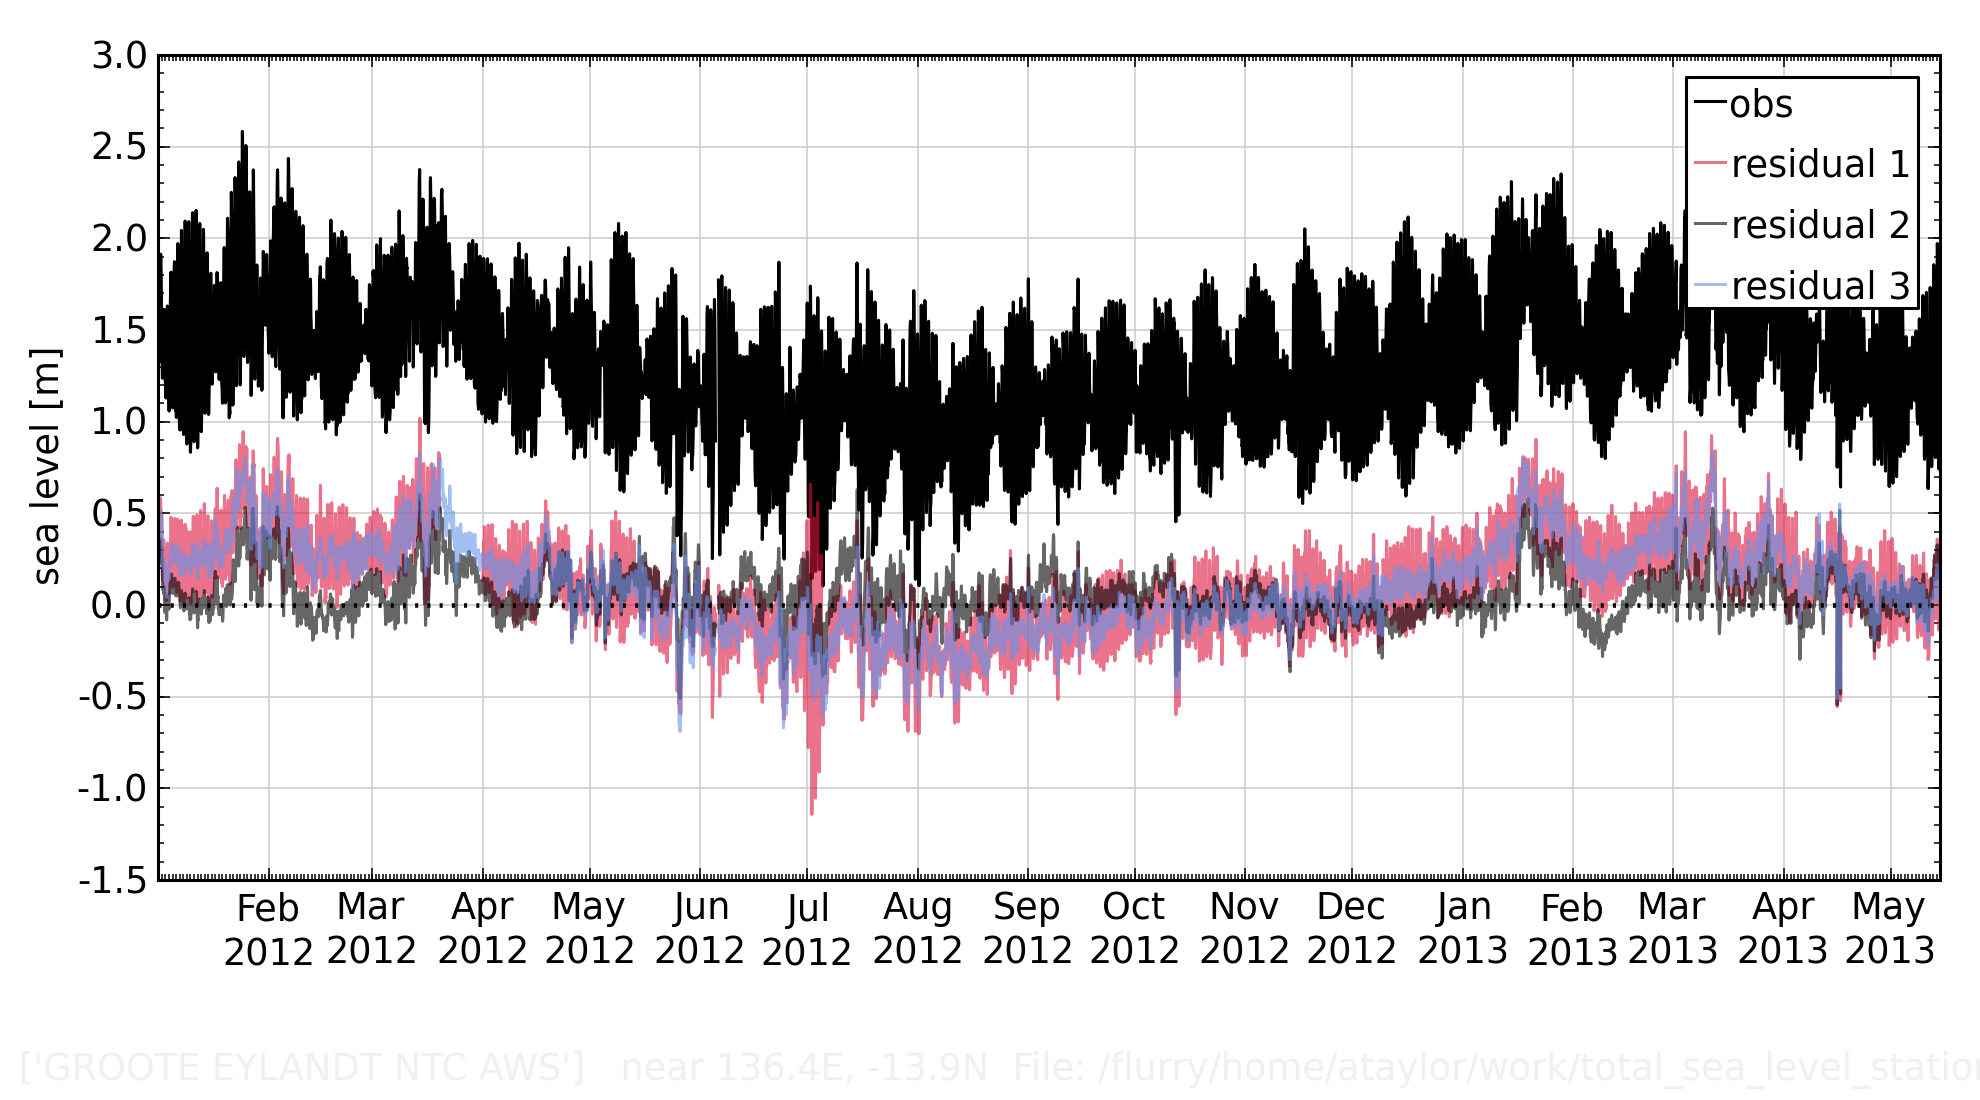
\includegraphics[width=\figwidthFull]{figures/plots/diag_plot_014406_detide_compare_20120101.png}
    \caption{Observations de-tided using alternate references.}{Different `residuals' result from alternative tide predictions: [1] regional gridded tide solution, [2] harmonic prediction and [3] harmonic prediction with significant non-gravitional harmonics removed. }
    \label{fig:residualExample}
\end{figure}
%-------------------------

%-----------------%
\subsection{Global tides}
\label{sec:spatialTides}
Extending the basic premise of tidal analysis to the whole ocean results in a global tidal atlas.  A tide atlas, or global tide solution characterise the tidal admittance across the whole ocean surface; rather than just a single point.
Global tide solutions have been enabled by satellite altimetry.
Indeed, the design and motivation for satellite altimetry missions have been to a large degree driven driven by the study of ocean tides.
Meaningful tidal atlases existed prior to altimetry, most significantly that due to Schwiderski \citep{Schwiderski:1983ke}, but these necessarily suffered from a lack of validation and constraint in the deep ocean.


Global tide models are employed for a range of purposes beyond sea level forecasting,often as an intermediate step or a correction, for applications in gravity, orbit determination, earth rotation and even the definition of coordinate systems \citep{IERS2003}.

Most importantly for the present discussion, global tide models are employed to filter, or ``de-tide'', sea level observations from near-real-time altimetry as a data assimilation constraint on mesoscale ocean forecast models.   This topic is discussed further in section \ref{sec:mesoscaleOperational}.


The typical visualisation of a tidal atlas is in the form of maps of time-invariant tidal amplitude and phase for a sequence of named constituents; regardless of whether a harmonic method was actually employed to produce the solution.   Each map describes a component wave or ``partial tide''.  These are maps are also called `co-tidal' and `co-range' plots.
In line with the discussion in section \ref{sec:LTI}, whole ocean is conceived as a LTI system. 
The long spatial scale of these component waves and the existence of spatial nodes places special importance upon amphidromes or amphidromic points - nomenclature introduced by Harris in the late 19th century \citep[pp 119]{Cartwright:2000tt}.  Existence and placement of amphidromic points is an important visual metric employed to assess tidal model results.  
Figure \ref{fig:atlas} shows a typical tidal atlas map for a single constituent with amphidromic systems apparent as radial patterns in the co-phase diagram.

Modern tidal atlases are in close agreement with regard to broad patterns, but characteristically differ at the shallow water margins; the very location of most direct interest to sea level forecasts.  Figure \ref{fig:tpx_cross} illustrates the fact that modern global tide models typically agree within about 0.02m in the deep ocean, but can differ substantially in coastal and shelf regions.  
%---------------------------
\begin{figure}[!hbt] \centering
    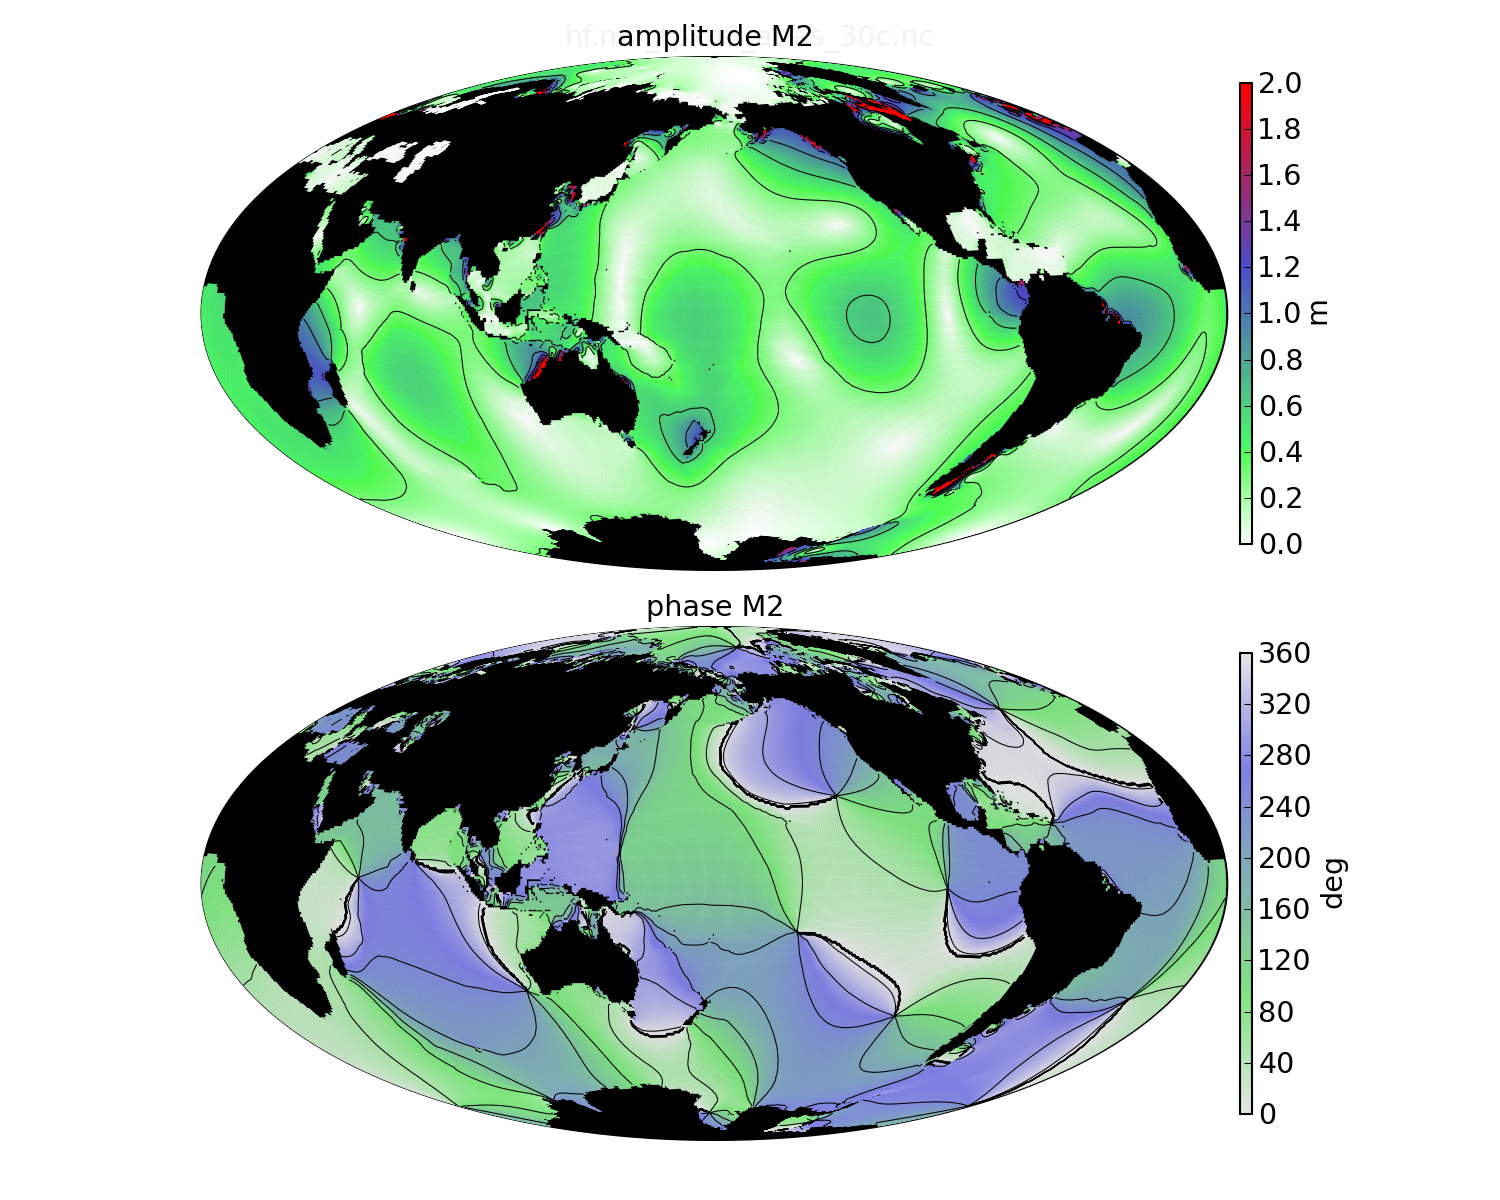
\includegraphics[width=\figwidthBig]{figures/maps/global_m2_tpx08.png}
    \caption{Tidal cophase and corange diagram.}{Example spatial snapshot for a single tidal component M2.  Data source TPX08 \citep{Egbert:2002ug}  }
    \label{fig:atlas}
\end{figure}
%---------------------------
\begin{figure}[!hbt] \centering
    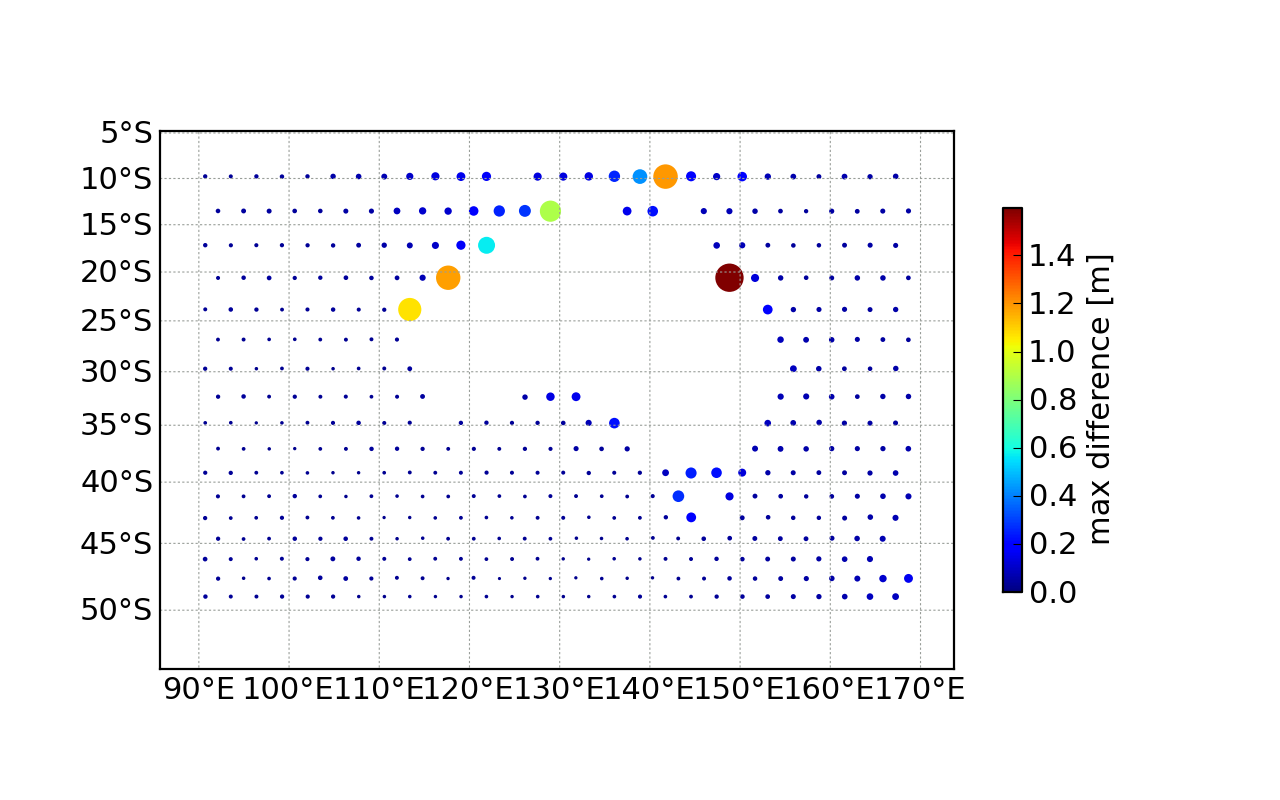
\includegraphics[width=\figwidthBig]{figures/maps/map_tide_differences_tpx_xovers.png}
    \caption{Tide solution differences at topex cross-overs near Australia.}{Maximum absolute differences between tidal timeseries at topex cross-overs for a 1 year period. The different solutions agree very closely in deep water, whilst the significance of shallow water effects are apparent.  Models included: CSR04\citep{Eanes:1996tr}, FES04\citep{Lyard:2006ir}, DTU10\citep{IMPROVEMENTOFGLOBA:2010tu}, GOT47, GOT48\citep{Schrama:1994vr}\citep{Ray:1999vm} }
    \label{fig:tpx_cross}
\end{figure}
%---------------------------
%TBC 
%Altimetry has directly enabled contrasting scientific developments in global tides (eg.\citet{Egbert:1996vr},  \citet{Lefevre:2011dg}) and mesoscale ocean variability (eg.  \citet{Wunsch:1998bq}, \citet{Chelton:vi}).
The LTI concept embodied in tidal atlases is well suited to representing deep water tides.   Amplitudes of each partial tide are no larger than about 0.02 cm for the majority of the global ocean, compared to depths of around 4km.
Given the underlying LTI framework, the tidal literature has naturally focused on stationary frequency-space metrics.  Intercomparison of mode1s and assessment against observations is almost always performed at a small set of dominant tidal frequencies - commonly only M2, K1, O1 and S2.

Summaries that categorise the many global tide models on the basis of design choices, parameterisations and data assimilation methods are given in \citep{Ardalan:2008gs} and \citep{Matsumoto:2000tg}. 

Tidal atlases are in essence spatial extensions of insitu tide predictions and subsequently each solution is formulated in terms of a particular tidal formalism.  
Similarly, interpretation of any tidal atlas warrants special attention to be given to the representation of signals associated with non-gravitational effects.   This topic is discussed further in chapter \ref{chp:tideFlavours}.


Some authors have gone so far to presented the existence of repeat-orbit altimetry observations as effectively being `thousands of tide gauges', but reduction of these observations via tidal analysis requires many special considerations. Most obviously is that ground-path of these orbits results in repeated but infrequent samples of any fixed point; and subsequently frequency aliasing is a primary limitation on tidal analysis methods..



Despite the general equivalence, a point of practical difference is the treatment of the non-linear effects significant in shallow water.
In contrast to the apparent convergence of surface tide models in the open ocean, shelf and coastal regions are problematic.   In shallow waters wavelengths shorten and nonlinear interactions between partial tides can become very prominent. 


A strength of conventional 1-dimension analyses of coastal tide gauges has been the incorporation of shallow water compound tides.  It is not atypical in Australian locations to include dozens of nonlinear frequencies in a harmonic analyses.   Nonlinear signals observed at a tide gauge are often attributed to complex very localised dynamics.  
Understandably, global tidal atlases in optimising the linear deep water signal and have relatively poorly represented or ignored coastal nonlinearties.  The nonlinear M4 signal (associated with self-interaction of M2 waves) is perhaps the only such partial tide to be included in many modern atlases and is observable with altimetry \citep{Ray:2010jm}.


As a forecast product, tidal atlases have nothing like the broad economic integration of conventional coastal tide tables.  The Australian Bureau of Meteorology does not promulgate official tide predictions away from insitu observation locations. 
For the contemporary operation setting, tidal atlases are primarily relevant as an intermediate product to enable satellite observations and to apply as open boundary condition forcing to downscaled simulations.


Coordinated development of improved tidal atlases with specific performance requirements formed a significant component of altimetry missions in the 1990s.
\begin{quotation} \noindent
This international effort quickly split into two main approaches: the so-called empirical approach based on the direct analysis of the altimetry sea level time series \dots{}, and a modelling approach based on hydrodynamic and assimilation models. Later on, the interaction between the two approaches (i.e. data assimilation based on altimetry analysis on one hand, and hydrodynamic/assimilation modelling on the other hand) was a key factor for the overall success in improving tidal prediction accuracy and reaching the T/P requirements \citep[pp394]{Lefevre:2011dg}.
\end{quotation}

No global tidal atlas can be empirical to the extent of simple timeseries analysis - the spatial and temporal coverage of observations are too sparse.

Schwiderski's pre-altimetry solutions relied heavily on global compilations of harmonic constants for mainly coastal tide gauges, from which spatial maps were created via a `hydrodynamic interpolation' method that would in hindsight be considered an application of data assimilation \citep[pp822]{Egbert:1994wz}.

Now with over 20 years of altimetry data, all the highly evolved global tidal models or tidal solutions employ \underline{data assimilation} in some manner.  That is, they make some combined use of dynamic models and observational data.  
The data assimilation employed for global tide solutions has quite a different form to that used in forward models like \BL{}; section \ref{sec:mesoscaleOperational}.  Whereas a mesoscale ocean model requires initial conditions from which to integrate forward in time, the LTI tidal conception of the ocean seeks a single optimal solution in frequency space. 


The dynamics relevant to tidal sea level are conventionally written as the Laplace Tidal Equations (LTE) ; \citep[9.8]{gill1982atmosphere} and \citep{Hendershott:1981ub}.  The LTE are a set of depth integrated shallow water equations on a rotating thin shell.  Advection is neglected altogether.
The combination of barotropic hydrodynamics and data assimilation used in global tide models has proven to be a adequate when the aim is to map tidal patterns of surface elevation.  The LTE provide a tractable means of doing so given the incomplete spatial and temporal coverage of observations.
This formulation excludes a direct representation of internal tides, despite the important role they play in the energetics of ocean tides.
\begin{quote}
    Barotropic tides generate internal tides, and internal tides in turn feed back onto the barotropic tides. Inferences from altimetry-constrained barotropic tide models show that about one-third of global tidal energy dissipation occurs in regions of rough topography, where internal tides are generated \dots{}. Internal tide generation thus acts as a damping mechanism for the barotropic tides.\citep[pp22]{Arbic:hy}
\end{quote}
Depth integrated barotropic LTE relegate the effect of internal mechanisms on surface elevation to parameterisations.  The dissipative stress term (F in equation \ref{eq:LTE_momtm}) stands for all losses of energy from the barotropic simulation.  Given the reality of ocean stratification, this loss term accounts for the conversion of barotropic to higher baroclinic modes in any global solution \citep[pp121] {gill1982atmosphere}.
Internal waves at tidal frequencies do have an observable surface signature albeit relatively small \citep{Ray:2011tj}.  
For sea level forecasting, internal modes are ostensibly of interest insofar as they impact the prediction of surface elevation.  
Internal tides are in general not stationary and not as predictable as surface tides \citep{Nash:2012}.  The extent to which aperiodic internal modes can be separated from surface tides is a measure of the value core stationarity model of  tide prediction.
The tidal view of the ocean as a LTI system driven by the \ATGP{} is very useful, but with the caveat that ``the ocean is a physically complex and noisy filter.  In consequence, tidal harmonics are not strictly constant \citep[197]{Ray:2010jm}''.  
Whilst stratification and all internal hydrodynamic mechanisms are very coarsely parameterised in global tide models, the internal structure of the ocean is a primary focus of \OGCM{}s, and this forecasting perspective is discussed in section \ref{sec:mesoscaleOperational}.  Some further detail on modelling global tides is also included in Appendix \ref{appendix:globalTides}.

%-----------------%
\subsection{Operational need for multiple tide concepts}
The above sections have portrayed the ways that ocean tides have come to be employed for operational forecasts.
In the simplest terms, there are two operational conceptions of what ocean tides actually are;
\begin{itemize}
    \item tides as a predictable periodic variation in total water height and;
    \item tides as a longwave physical response to gravitational forces.
\end{itemize}
Whereas methods for representing and forecasting both of these are centred on the linear-time-invariant concept of an ocean admittance, they are not identical.
Furthermore, the aim of forecasting the total water height differs greatly in intent from the aim of filtering or decomposing water height; and there is no reason to require both to be satisfied by a single conceptualisation of an ocean tide. 
Allowing for ocean tides to be other than singular may give rise to some unique complications given that conventional tide predictions have come to play such an established role in coastal economies.   A notable role in this regard is how derivations from conventional tide predictions are built into spatial references such as nautical chart datum and highest astronomical tide (HAT).   Ensuring that forecast products are consistent with these spatial applications would appear to require some care.  
Most broadly, there is room in the operational setting for improved clarity in handling tides in forecasting and this topic is addressed in both chapters 
\ref{chp:aggregate} and \ref{chp:tideFlavours}. 
